\documentclass[11pt,a4paper]{article}
\usepackage[T1]{fontenc}
\usepackage[utf8]{inputenc}
\usepackage[margin=22mm]{geometry}
\usepackage{graphicx,longtable,booktabs,amsmath,array}
\usepackage[colorlinks=true,urlcolor=blue,linkcolor=teal,citecolor=teal]{hyperref}
\usepackage{microtype}
\setlength{\emergencystretch}{3em}
\title{Initial Reproduction Report}
\author{Muhammad Sameer \and Humayun Bilal\\\small Cloud Computing Research Project}
\date{7 October 2026}
\begin{document}
\maketitle
\noindent\textbf{Manuscript note:} Author names follow the predecessor proposal. Confirm affiliations, student IDs and contributions before submission. Mentor approval is reported by the team; this source does not assert final manuscript acceptance. The official course/journal template was not supplied.

\textbf{A Data Rate Monitoring Approach for Cyberattack Detection in Digital Twin Communication}


Prepared by Muhammad Sameer and Humayun Bilal  Cloud Computing Research Project  7 October 2026


\section{Abstract}

This report evaluates the reproducibility of a recent MQTT digital-twin security study using its official source code. The original MQTT functions were executed through a native adapter, followed by the authors' Docker services and bounded intrusion, command-modification and denial-of-service scenarios on Linux. Calibration completed, manipulated commands stopped simulated sensors, and the bounded flood triggered rate alerts. Exact numerical replication was not possible because the original traces were not available and the published method differs from the released implementation. This report records those differences, the executed environment, data provenance and limitations. The subsequent methodology report evaluates a separate freshness-aware recovery contribution; its results are not attributed to the reference article.


\section{Reference and project identification}

\begingroup\small\setlength{\tabcolsep}{3pt}\begin{longtable}{p{0.44\linewidth}p{0.44\linewidth}}	oprule
Field & Verified information \\
\midrule\endhead
Paper title & A Data Rate Monitoring Approach for Cyberattack Detection in Digital Twin Communication \\
Paper authors & Claudio Rodrigues; Waldir S. S. Junior; Wilson Oliveira; Isomar Lima \\
Venue and year & Sensors, volume 25, issue 24, article 7476; 2025 \\
Publication date & 9 December 2025 \\
Paper link & \href{https://doi.org/10.3390/s25247476}{Publisher/DOI} \\
Accessible full text & \href{https://pmc.ncbi.nlm.nih.gov/articles/PMC12736672/}{PubMed Central} \\
Official source repository & \href{https://github.com/woliveira1728/digital-twin}{woliveira1728/digital-twin} \\
Executed source revision & 43346f60a9f41392611242ff3cb7589d7a758aa7 \\
Student research repository & \href{https://github.com/SMR202/dt-mqtt-resilience}{SMR202/dt-mqtt-resilience} \\
Research changes and evidence & \href{https://github.com/SMR202/dt-mqtt-resilience/pull/1}{Research PR \#1} \\
\bottomrule\end{longtable}\endgroup

The article links the official repository in its data-availability statement; the repository README identifies the same article. The selection meets the requirement for an executable, author-linked research artifact. Sensors is a peer-reviewed journal; this report does not describe it as a top-tier systems venue. The paper is relevant to the project's MQTT communication and digital-twin resilience topic. The feasibility audit and alternative-paper assessment remain in \texttt{docs/INITIAL\_REPRODUCTION\_AUDIT.md}.


\section{Problem, approach and architecture}

The paper addresses attacks on the communication channel between simulated industrial devices and their digital twins. Its proposed monitor uses communication-rate changes to detect anomalies without interpreting individual payloads. The stated statistical threshold is the normal rate mean plus three standard deviations. The study evaluates denial of service, active man-in-the-middle command modification and intrusion that stops sensor activity.


The logical architecture consists of a simulated device, MQTT broker, digital-twin service and monitoring service. The device publishes sensor readings; the twin receives data and sends commands through the broker. Attack components invoke the twin's HTTP interface or intercept commands through a proxy. Docker separates services and supplies a repeatable deployment topology. The released monitor counts MQTT callbacks and payload bytes; this measurement boundary differs from the paper's packet/byte-rate terminology.


The cloud computing component is the containerized communication and twin service stack, which is deployable on a cloud host. The published experiment describes a controlled Docker host, rather than a verified AWS/Azure deployment. Our later AWS experiment is a separate extension. There is no multimodal learning component: multiple synthetic sensor channels are telemetry attributes, not an image/audio/text fusion dataset.


\begin{figure}[htbp]\centering\IfFileExists{figures/baseline_architecture.png}{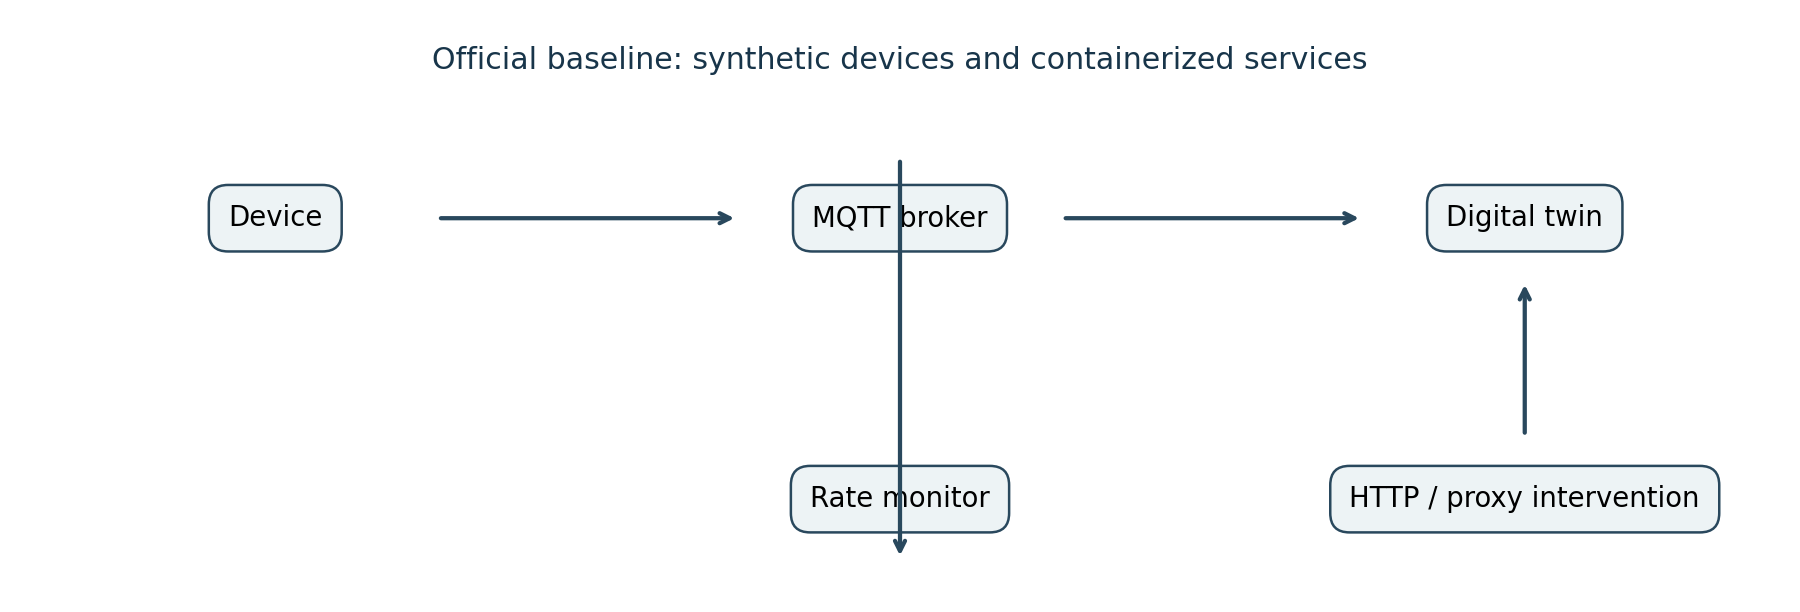
\includegraphics[width=.95\linewidth]{figures/baseline_architecture.png}}{\fbox{\parbox{.85\linewidth}{Upload figures/baseline\_architecture.png to display this figure.}}}\caption{Logical baseline architecture. Telemetry traverses the broker; the monitor observes communication and controlled interventions affect commands.}\end{figure}

\section{Data inventory and preparation}

\begingroup\small\setlength{\tabcolsep}{3pt}\begin{longtable}{p{0.29333333333333333\linewidth}p{0.29333333333333333\linewidth}p{0.29333333333333333\linewidth}}	oprule
Dataset or trace & Source and size & Characteristics and use \\
\midrule\endhead
Authors' synthetic device telemetry & Official device generator; original recording files and total record count not released in the inspected artifact & Simulated industrial sensor readings and commands; normal calibration and controlled attack periods \\
Published scenario statistics & Paper Table 2; six normal/attack rows & Aggregate means and standard deviations; reference values only, not raw input data \\
Native reproduction trace & Original MQTT functions through our adapter; 283 observer events, including 200 benign burst sensor messages & Timestamped messages and calibration/control events; raw events, source hashes and logs retained \\
Docker reproduction logs & Original services; successful calibration and three bounded scenarios & Timestamped device, proxy and monitor logs; scenario execution records and compressed service logs retained \\
Additional local MQTT comparison & Our extension; 108 runs and 51,840 generated/audited updates & Four synthetic devices, three QoS levels and controlled application-level conditions; separate from baseline replication \\
Additional Linux impairment comparison & Our extension; 36 runs, 4,248 generated/audited updates & Actual local TCP packet impairment; raw PCAP, qdisc counters, receipt events and audit snapshots \\
Additional cloud comparison & Our extension; 36 runs, 14,256 generated/audited updates and 3,709 unique cloud receipts & Actual PC-to-AWS transport with synthetic input; not physical sensor data \\
\bottomrule\end{longtable}\endgroup

There are no train/validation/test splits because the reference is a traffic-monitoring experiment, not a trained machine-learning model. Normal/calibration and intervention windows serve different experimental purposes and must not be described as ML splits. The article describes a 60-minute healthy capture, while Table 2's caption identifies a normal interval before 40 seconds; these descriptions do not establish the size of an accessible dataset. The released device calibration lasts approximately 66 seconds. Without the original traces, their precise relationship cannot be reconstructed.


Preparation preserves generated values and records device/sequence identifiers, timestamps and scenario boundaries. Log analysis counts new events within each intervention window rather than treating cumulative log totals as new outcomes. Additional synchronization experiments retain append-only local SQLite audit histories and independently match received samples to generated records. No missing author samples were imputed, no external dataset was substituted as the authors' original data, and no outliers were removed to improve results. The source does not provide a reproducible random-seed protocol for its published attack figures; our extension records its own seeds and configurations.


\section{Hardware, software and cloud resources}

\begingroup\small\setlength{\tabcolsep}{3pt}\begin{longtable}{p{0.29333333333333333\linewidth}p{0.29333333333333333\linewidth}p{0.29333333333333333\linewidth}}	oprule
Component & Published or released environment & Executed environment \\
\midrule\endhead
Host hardware & Precise CPU model, RAM and physical-device specifications not located & AMD x86-64 desktop; six physical/12 logical CPUs; approximately 16GiB RAM; no GPU or physical sensor used \\
Operating system & Ubuntu 24.04.3 LTS & Native Windows build 26200; Linux extension on Ubuntu/WSL2, kernel 6.18.40.1; AWS extension on Ubuntu 24.04.4 LTS \\
Python & Paper: 3.12; Dockerfiles: python:3.10-slim & Native 3.10.9; Linux comparison 3.10.22; cloud receiver 3.12.3 \\
Container runtime & Docker 28.4.0; Compose 2.39.4 & Private Docker 29.1.3 runtime; exact commands/build information retained in execution records \\
MQTT client & Paper: Paho 1.6.1; source uses a newer callback API & Paho-MQTT 2.1.0 \\
MQTT broker & Official Docker Mosquitto service & AMQTT 0.11.3 for native/local comparison; original broker container for source topology; Mosquitto 2.0.18 for AWS \\
Other baseline libraries & Paper: Requests 2.32.3, OPC-UA 0.98.13, aiocoap 0.4.3; Docker installs are mostly unpinned & Original Dockerfiles preserved; the native core runs MQTT only and does not claim OPC-UA/CoAP replication \\
Analysis libraries & Not specified for our analysis & NumPy 2.2.6, pandas 2.3.3, Matplotlib 3.10.7, psutil 7.1.0 \\
Cloud resource & No verified public-cloud benchmark in the paper & Separate temporary AWS t3.micro in Stockholm: two vCPUs, 1GiB RAM, 8GiB gp3 root storage; SSH-restricted access and localhost-only MQTT \\
\bottomrule\end{longtable}\endgroup

Full dependency versions are in \texttt{requirements-lock.txt} and experiment environment files. The executed Docker images use the authors' unchanged Dockerfiles, whose unpinned dependencies prevent claiming the exact 2025 package environment. Source provenance is preserved through the pinned Git revision and recorded Python-file hashes.


Important baseline settings include one-second application-rate observations, approximately 66 seconds of source calibration, and controlled HTTP/proxy interventions. The successful Docker topology uses an internal bridge, explicit service host mappings, no published host ports, a broker-first startup and 0.5 CPU/256MiB service limits. The flood uses one worker for five seconds. These bounds differ from the original defaults and are part of the reproduction protocol. Further configurations remain in the delivered JSON files rather than being inferred from plotted outcomes.


\section{Published results and reproduced observations}

The following values are transcribed from the paper's Table 2. They are \textbf{published reference statistics}, not measurements produced by this project. The paper labels the rates PPS and BPS.


\begingroup\small\setlength{\tabcolsep}{3pt}\begin{longtable}{p{0.14666666666666667\linewidth}p{0.14666666666666667\linewidth}p{0.14666666666666667\linewidth}p{0.14666666666666667\linewidth}p{0.14666666666666667\linewidth}p{0.14666666666666667\linewidth}}	oprule
Scenario & Period & Mean PPS & SD PPS & Mean BPS & SD BPS \\
\midrule\endhead
DoS & Normal & 13.75 & 4.27 & 7,309.92 & 3,082.47 \\
DoS & Attack & 779.30 & 156.03 & 50,904.75 & 15,049.37 \\
MiTM & Normal & 12.70 & 4.59 & 7,085.28 & 2,656.04 \\
MiTM & Attack & 65.68 & 14.97 & 25,445.80 & 8,674.89 \\
Intrusion & Normal & 14.95 & 5.08 & 7,721.48 & 3,213.76 \\
Intrusion & Attack & 21.52 & 55.55 & 3,664.50 & 10,141.59 \\
\bottomrule\end{longtable}\endgroup

Our observations establish executable behavior, rather than equality with those statistics.


\begingroup\small\setlength{\tabcolsep}{3pt}\begin{longtable}{p{0.29333333333333333\linewidth}p{0.29333333333333333\linewidth}p{0.29333333333333333\linewidth}}	oprule
Reproduction & Observed result & Interpretation \\
\midrule\endhead
Native MQTT core & Calibration completed; 283 observer events; all 200 benign burst sensor messages observed & Core communication and calibration functions execute; the adapter required a completion-message resend \\
Rule comparison on native trace & Independent three-sigma threshold 3.2355 messages/s; observed maximum threshold 4 messages/s & The paper's rule and the source's maximum rule are different methods \\
Original Docker calibration & Completed without the native completion-message repair & Container topology executes after networking adaptations \\
HTTP injection & Three newly logged device sensor shutdowns & Command injection changes simulated device behavior \\
Command-modifying proxy & One newly logged modification and one sensor shutdown & The proxy path changes a command and affects a simulated sensor \\
Bounded HTTP flood & 1,033 new command receipts; 14 rate alerts; maximum reported command rate 237 application messages/s & Executed intervention produces elevated application traffic and alerts; not wire-packet or classification-accuracy evidence \\
\bottomrule\end{longtable}\endgroup

Raw observations are in \texttt{results/baseline\_core/} and \texttt{results/linux\_attacks\_attempt2/}; independent checks are in \texttt{results/processed/linux\_attack\_checks.json}. The unsuccessful Docker attempt remains in \texttt{results/linux\_attacks\_attempt1/}. No confusion matrix, precision/recall, accuracy, or numerical replication error against Table 2 is calculated because the necessary comparable traces and measurement boundary are unavailable.


\section{Differences, problems and explanations}

\begingroup\small\setlength{\tabcolsep}{3pt}\begin{longtable}{p{0.29333333333333333\linewidth}p{0.29333333333333333\linewidth}p{0.29333333333333333\linewidth}}	oprule
Category & Finding & Handling and effect on comparability \\
\midrule\endhead
Installation & Docker Desktop's engine did not start & Official Ubuntu packages were extracted into a private Linux runtime; no system Docker service was installed \\
Networking & Initial container service DNS failed & Preserved the failed logs; successful rerun uses explicit private service addresses/host mappings \\
Code/API & Source uses CallbackAPIVersion, absent from the paper's specified Paho version & Used Paho 2.1.0 and disclosed the version mismatch \\
Method & Released rate monitor compares calibration maxima; paper specifies mean plus three SD & Preserved source behavior and implemented the paper rule separately; did not silently alter the baseline \\
Measurement & Source counts MQTT application callbacks and payload bytes & Reported application rates; did not relabel them as wire packet counts \\
Control delivery & Native calibration completion message was lost before disconnect & Adapter resends only this control message with an active network loop and QoS1; original method bodies remain unchanged \\
Logging & Unicode arrows conflicted with Windows default encoding & Native logs use UTF-8 \\
Dataset & Original CSV/PCAP, exact total recording size and repeated-run seeds were not located & Generated new traces, preserved actual counts and marked exact numerical replication unavailable \\
Missing resources & No original CPU/RAM details or physical sensors supplied & Recorded actual desktop/cloud resources and used synthetic devices \\
Computational limits & Desktop scheduling, short horizons and service caps affect throughput & Reported measured resource use; avoided general hardware-performance claims \\
Deviations & Native MQTT-only adapter; later bounded Docker scenarios; shorter recording; changed runtime/dependencies & Each stage is labeled independently; none is presented as full replication of every protocol or published figure \\
Licensing & No project-level upstream license located & Author source is fetched into ignored local work; it is not redistributed or relicensed as student code \\
\bottomrule\end{longtable}\endgroup

The most plausible explanations for rate differences are the changed observation boundary, duration, dependency/runtime versions, attack worker count and resource limits. Missing traces prevent separating those effects quantitatively. Successful execution supports the feasibility of the original architecture and selected mechanisms; it does not verify the paper's complete numerical findings.


\section{Research gap and next-stage methodology}

The reproduced code monitors traffic and prints received data but does not define sequence-safe current-state recovery. A high message count therefore cannot establish that the twin represents the newest device state. Our contribution evaluates a latest-state edge outbox, fair dispatch and a monotonic receiver against FIFO replay, while retaining a separate local audit record. This addresses freshness during backlog and recovery; it is distinct from attack classification.


The final report supplies architecture, metric definitions, configurations, ablations, comparative experiments and measured runtime/resources. Existing age-of-information literature already motivates update replacement, so novelty is framed as a reproducible MQTT recovery evaluation rather than invention of the underlying scheduling principle. Sensor hardware is optional for this scoped study and no physical-validation or energy claim is made.


\section{Reproduction and artifact access}

Begin with the official revision recorded in \texttt{baseline/manifest.json}. \texttt{scripts/fetch\_baseline.py} retrieves it privately; \texttt{scripts/reproduce\_core.py} runs the native core and \texttt{scripts/run\_linux\_baseline.py} runs the isolated Docker scenarios. Use a fresh output directory. Installation and evidence-verification instructions are in \texttt{docs/REPRODUCING.md} and \texttt{docs/LINUX\_EXTENSION.md}.


The student repository contains our original code, configuration files, execution records, raw/processed results and report sources. The baseline, proposed method and supplementary scenarios are separate artifacts. Instructor/mentor approval is reported by the team. Names, affiliations, student IDs, the official course template and final submission must be reviewed by the authors before delivery to the instructor.

\begin{thebibliography}{99}
\bibitem{ref1} Rodrigues, Junior, Oliveira, Lima. A Data Rate Monitoring Approach for Cyberattack Detection in Digital Twin Communication. Sensors (2025). \url{https://doi.org/10.3390/s25247476}.
\end{thebibliography}
\end{document}
